%================================================================================
%=============================== DOCUMENT SETUP =================================
%================================================================================

\documentclass[lang=english,inputenc=utf8,fontsize=10pt]{ldvarticle}
%PACKAGES

\usepackage{parskip}
\usepackage{subfig}
\usepackage{ifthen}
\usepackage{comment}
\usepackage{color}
\usepackage{colortbl}
\usepackage{soul}
\usepackage{tikz}
\usepackage{float}
\usetikzlibrary{shapes,arrows}
\usepackage{tabularx}
\usepackage{lipsum}
\usepackage{subfig}

\definecolor{lightgray}{rgb}{0.75,0.75,0.75}


%================================================================================
%================================= TITLE PAGE ===================================
%================================================================================

\title{Prediction of confirmed, recovered and death cases produced by COVID-19}
\author{Bueno Ulacia, Ion\\
Telecommunications Engineering\\
03726897
\and
Martín Cruz, Daniel\\
Telecommunications Engineering\\
03727385
}

\date{TU Munich \\ \today}


\begin{document}


\maketitle
\thispagestyle{empty}

\hrule


\tableofcontents

\vspace*{1cm}
\hrule

\newpage


% introduce the problem area, and define the question
\section{Introduction}
COVID-19 is currently the biggest challenge our generation has to face. It is necessary that governments all around the world work hard in stopping this global pandemic to save as many lives as possible in an efficient way so that economy does not experience a tremendous.

This is why our motivation for this project was to evaluate how good or bad was the management of different governments. We selected diverse scopes to provide a variety of views; a county, a region, a country and the whole world. The places we will study in this project are the following: Miami-Dade county, Bavaria, Brazil and the world. We chose Miami and Brazil because coronavirus had a strong impact there and Bavaria because it was one the first regions to suffer this disease.

Python and machine learning are great tools to make the evaluation of the management of the crisis. Our idea was to predict different coronavirus statistics from a certain point in time and compare them with the actual statistics. If the observed statistics are better than the predicted ones we can say that their management of the pandemic was better than expected and, on the other hand, if the observed values are worse than the predicted ones, we can say that it was a bad management.

In order to show the data we are using and our predictions we have developed a \textbf{dashboard} in which all these plots and statistics can be dynamically accessed and compared. In the report it is only presented some of these graphs.


% explain which data you use (cite the source appropriately!). Also take some time to describe properties of features with histograms/images/....
\section{Data description}
We used a free access and daily dataset \cite{Bing_covid}. It shows us the number of confirmed, recovered and deaths cases of COVID-19, in different parts of the world. The geographical scope is very deep, from counties to countries, including a reference for the entire world. The data is being updated every day and the first date depends on the region.

In order to see a global view, we have plotted the number of confirmed, recovered and deaths cases in a world map. For each location we selected, we plotted previously the number of cases, in order to have a first intuition about how to interpret and predict the data. An example of these plots is shown in Figure~\ref{fig:data}.

It can be seen the areas where the COVID-19 has a bigger impact and the evolution in the cases with the time.

\begin{figure}[H]
	\centering
	\subfloat[Map of confirmed cases in the world]{
		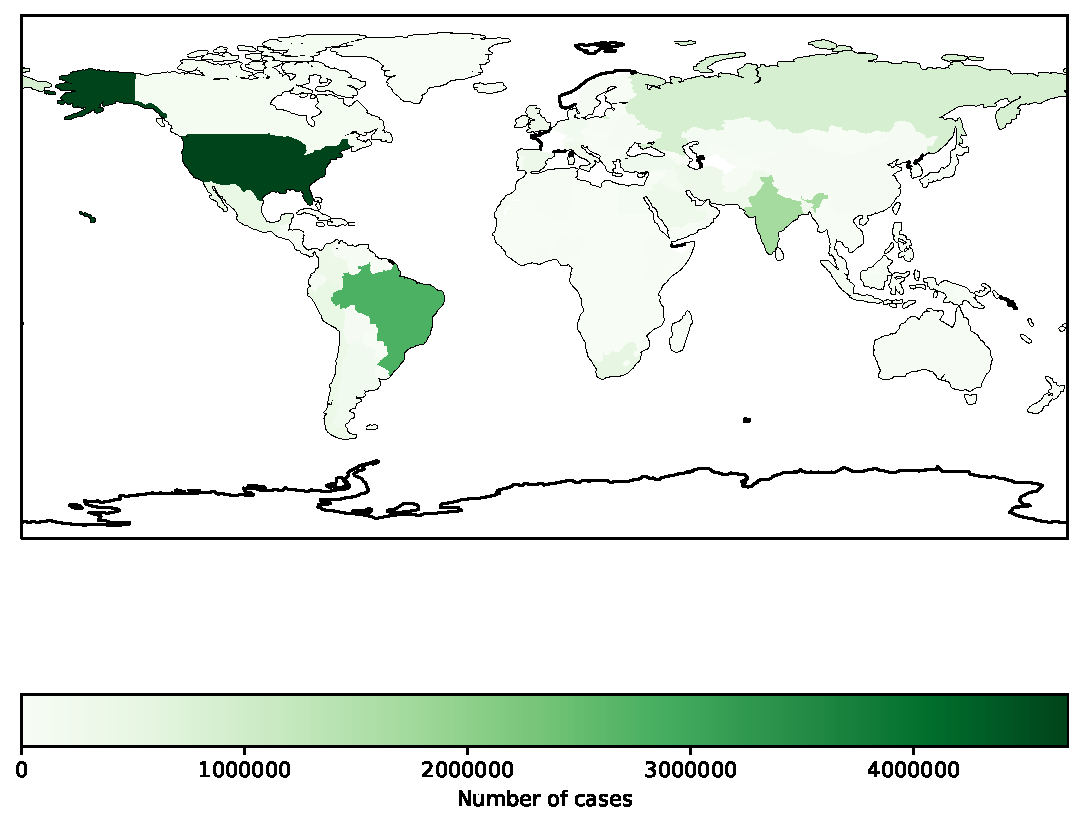
\includegraphics[scale=0.3]{plots/cases.pdf}}
	\subfloat[Confirmed, recovered and death cases in the world]{
		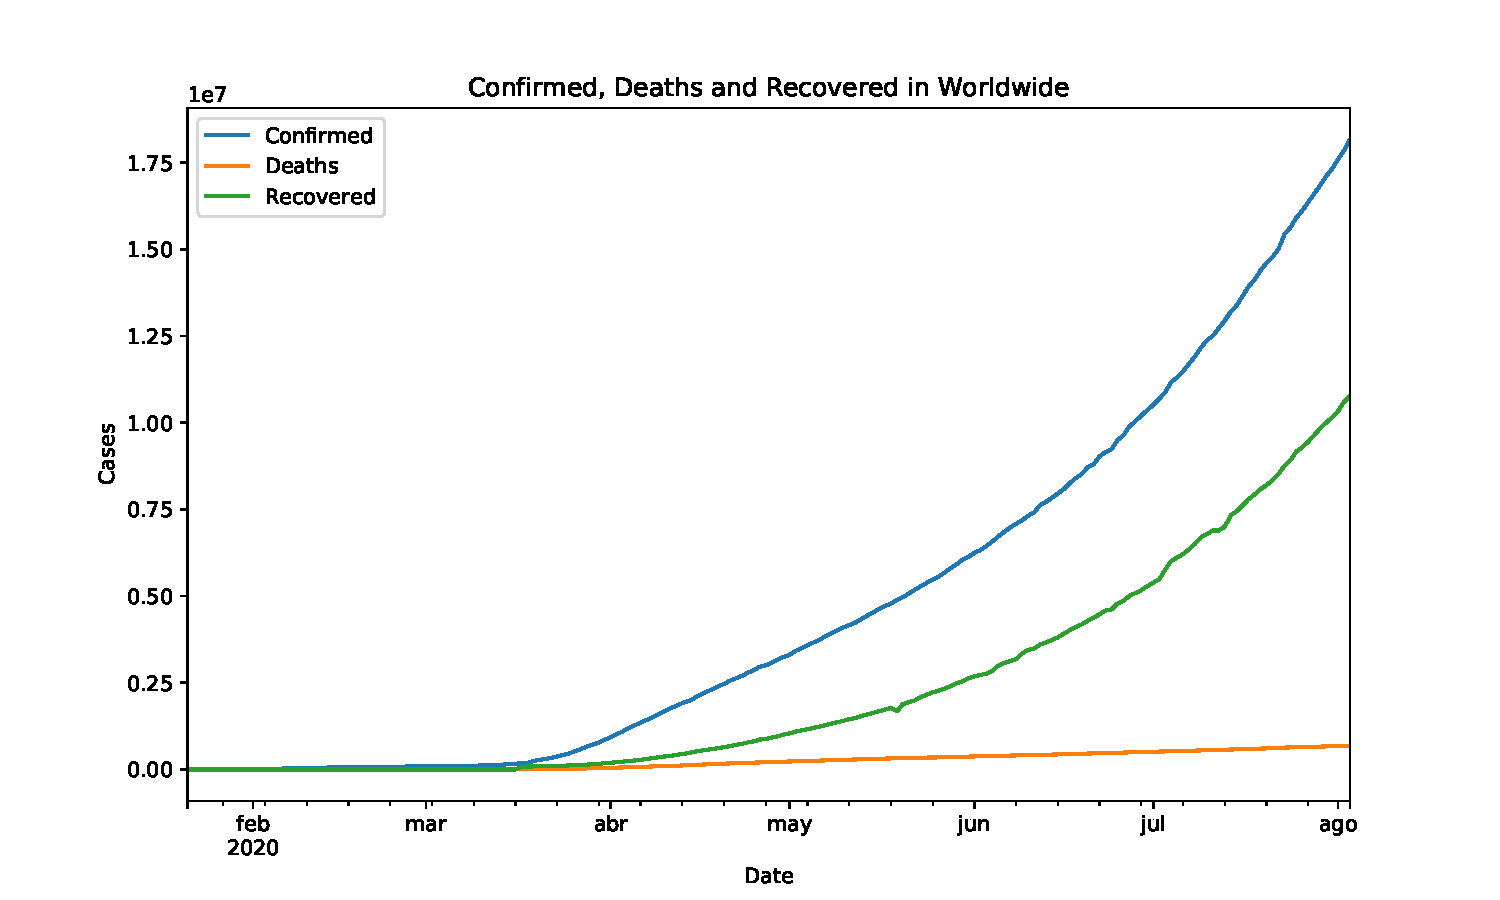
\includegraphics[scale=0.3]{plots/Worldwide_data.pdf}}
	\caption{Worldwide data}
	\label{fig:data}
\end{figure}



% outline which kinds of methods you are employing and which implementations you use (e.g. the major libraries you already got introduced to: tensorflow, keras, sklearn or new/other things - most of them offer a scientific citation!)
\section{Methods}
The goal is to see if the measures taken by the governments had an effect in the spreading of the virus. For this purpose, we predict the number of cases from a a determined point in the past, what means to perform a time series prediction.

We have used the ARIMA model. It is necessary to specify some parameters, for that reason, the model is really based in a different version of ARIMA, which is known as auto-ARIMA model \cite{auto_arima}. This one is distinguished for being an optimized version which looks for the optimal parameters. 
At first instance, the number of test samples is a quarter part of the total amount. This means we have employed three quarter parts of data to train, from the beginning date until the one which corresponds with the start of the last quarter amount. This parameter can easily be changed in the code.

In order to see the performance of the model, we used a predefined function \cite{plot_diagnostics} which shows us statistics about the residuals and estimated density.

These plots can be easily seen in the completed dashboard. The structure of the dashboard code can be divided in three parts:
\begin{itemize}
    \item 
    In the first we have all the python code where we generate all the necessary plots in an appropriate format for the dashboard, which is plotly. Here we have called all the already programmed methods used to produce data used to predict and the predictions of the coronavirus statistics.
    \item
    In the second part we have all the html code in which we are defining the final appearance of the dashboard. The dashboard is divided in three tabs in order to show used data, predictions and diagnosis of the predictions.
    \item
    In the third part of the code we have all the callbacks that are necessary so that the dashboard has a dynamic appearance, i.e. that we can select what type of data we want to plot: cases, deaths or recovered.
\end{itemize}
    

% Explain in detail the challenges you’ve faced and how you built the model (cross-validation, neural network layer architecture, loss, regularization, ...)
\section{Results}
The model is based in a time series prediction using an auto-ARIMA model. We have developed a model per location using the same machine learning algorithm. The main challenge is the model does not fit perfectly in every situation. This problem is not related with a big difference between the real and predicted data, since this would mean an impact of the taken measures.

To answer the original question we will focus on the confirmed cases data because the deaths and the recovered depend on more factors than only the governmental management like the mean age of the population or the health system of the corresponding country. We will answer the question with respect to the different chosen scopes:
\begin{itemize}
    \item 
    \textbf{United States, Florida, Miami-Dade County:} in the case of Miami we can see that they had a low number of cases in the early stages of the pandemic. We can see a clear inflection point around late June where the trend changed. We start the prediction in July and we expect that new trend but the rise is even worse than the predicted one. With this difference between expected and observed that measures taken in Florida were inefficient and probably they were executed late\cite{nbc_miami_2020}.
    \begin{figure}[H]
        \centering
        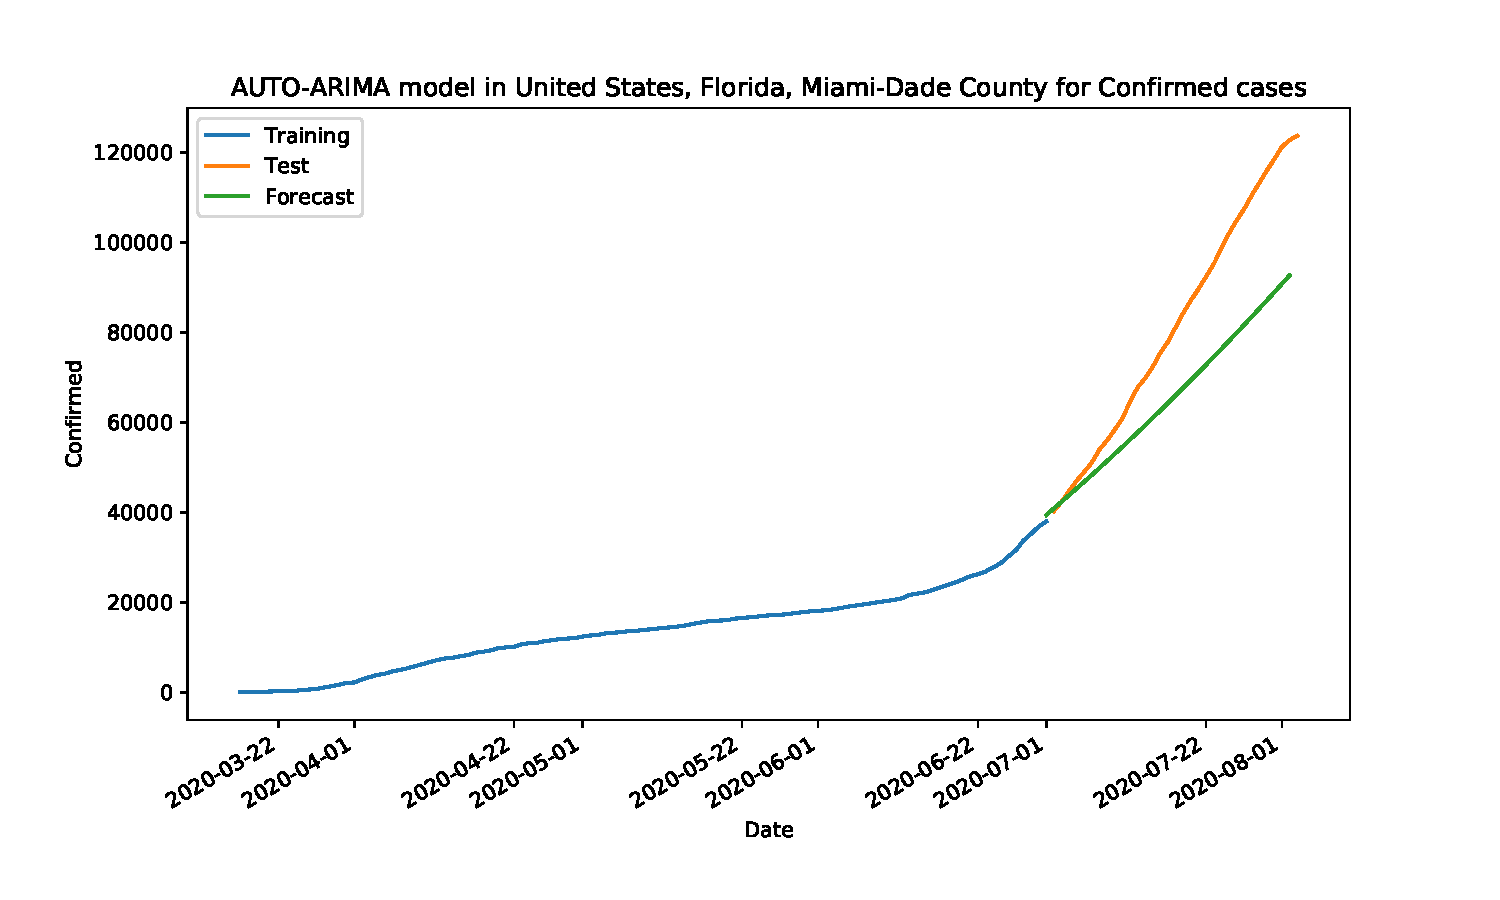
\includegraphics[scale=0.4]{plots/United_States_Florida_Miami-Dade_County_Confirmed_prediction.pdf}
        \caption{Prediction of confirmed cases in United States, Florida, Miami-Dade County}
    \end{figure}
    
    \item
    \textbf{Germany, Bavaria:} in this case, as it was already stated, we have a bad prediction for the confirmed cases in Bavaria so we cannot say much but looking at the data we collected. 	We can see the initial wave of new cases was stopped during May/April and from that point on the slope has remained constant which means that the management was correct.
    \begin{figure}[H]
        \centering
        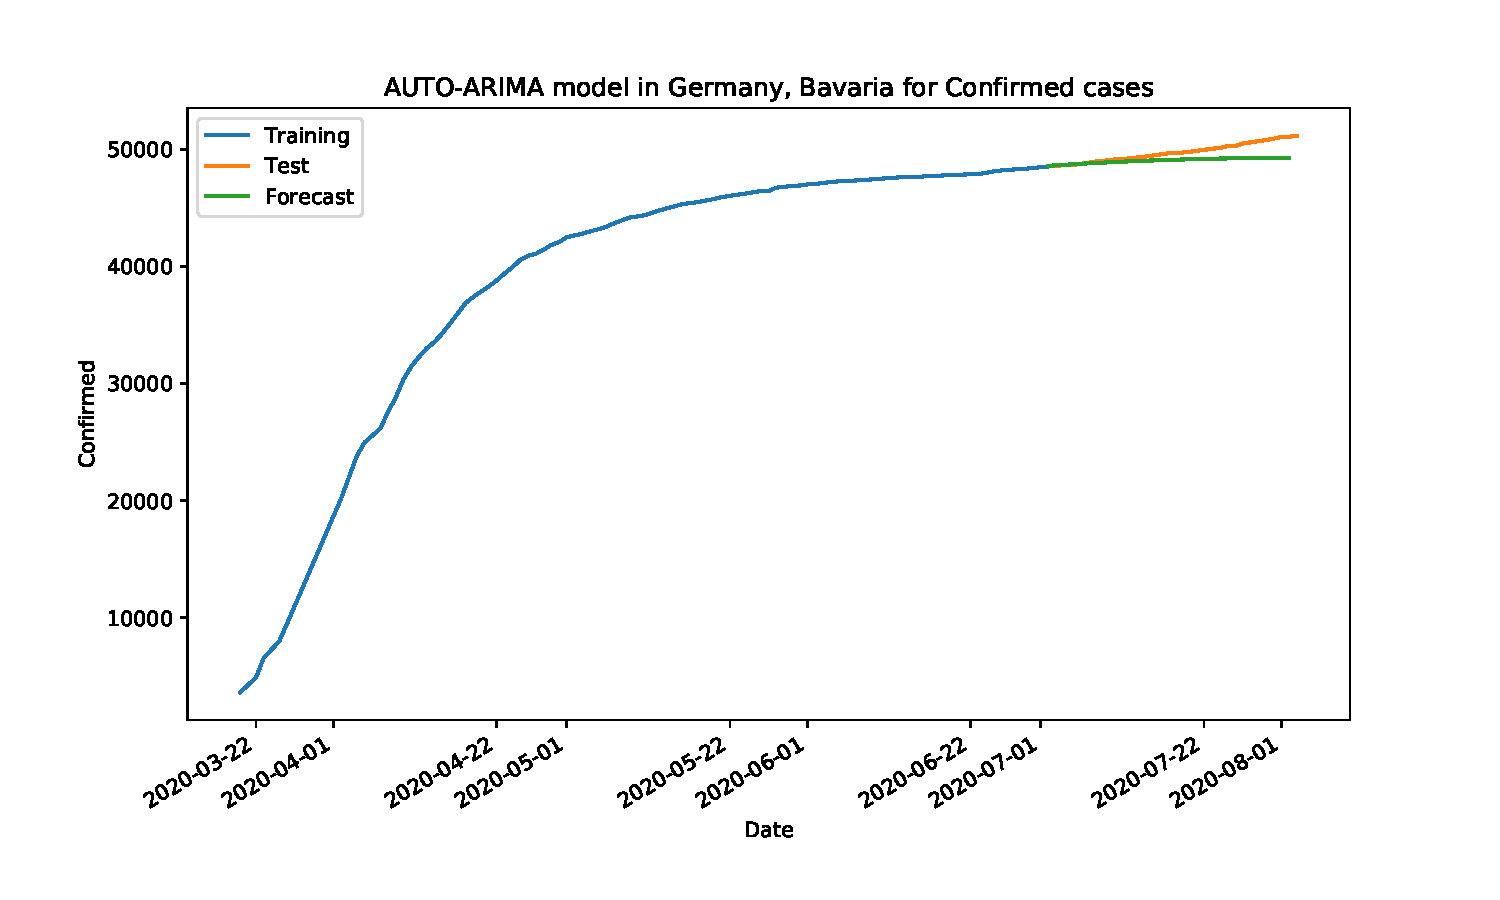
\includegraphics[scale=0.4]{plots/Germany_Bavaria_Confirmed_prediction.pdf}
        \caption{Prediction of confirmed cases in Germany, Bavaria}
    \end{figure}
    
    \item
    \textbf{Brazil:} watching to our prediction the expected and observed are similar, both with a considerable scope so it can be said the measures taken by the Bolsonaro's government has been as bad as the ones taken before July\cite{bbc_2020}
    \begin{figure}[H]
        \centering
        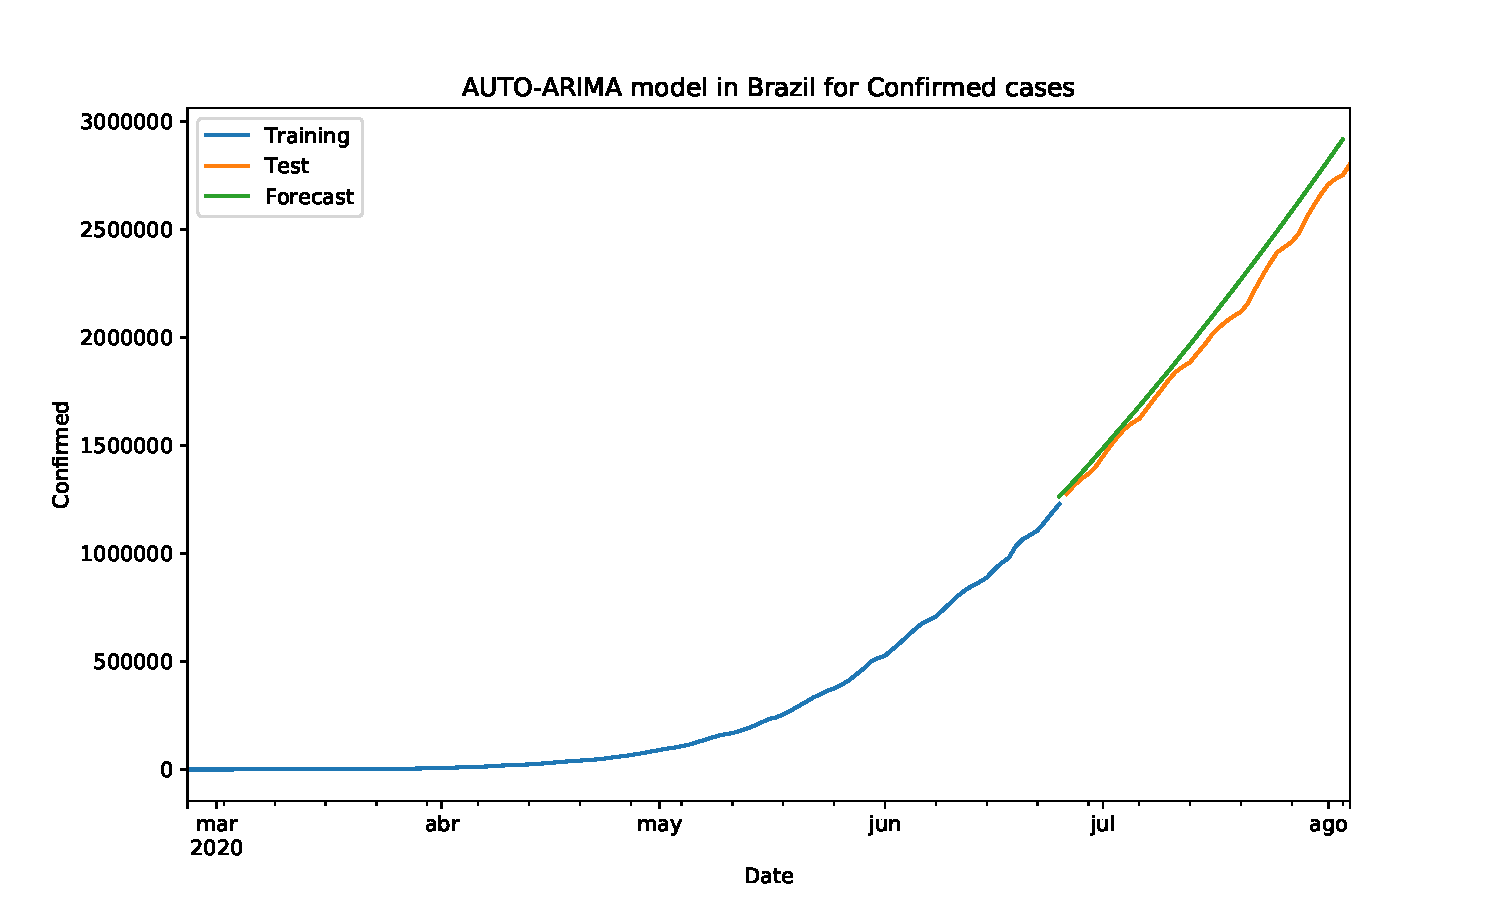
\includegraphics[scale=0.4]{plots/Brazil_Confirmed_prediction.pdf}
        \caption{Prediction of confirmed cases in Brazil}
    \end{figure}
    
    \item
    \textbf{World:} in the case of the overall confirmed cases the actual trend has been slightly higher than the predicted one. As it is the sum of the cases of every country we can't just say that management was good or bad but we may say COVID impact has been specially harder than expected in some countries like United Stated, Brazil and India\cite{theGuardian_2020}.
    \begin{figure}[H]
        \centering
        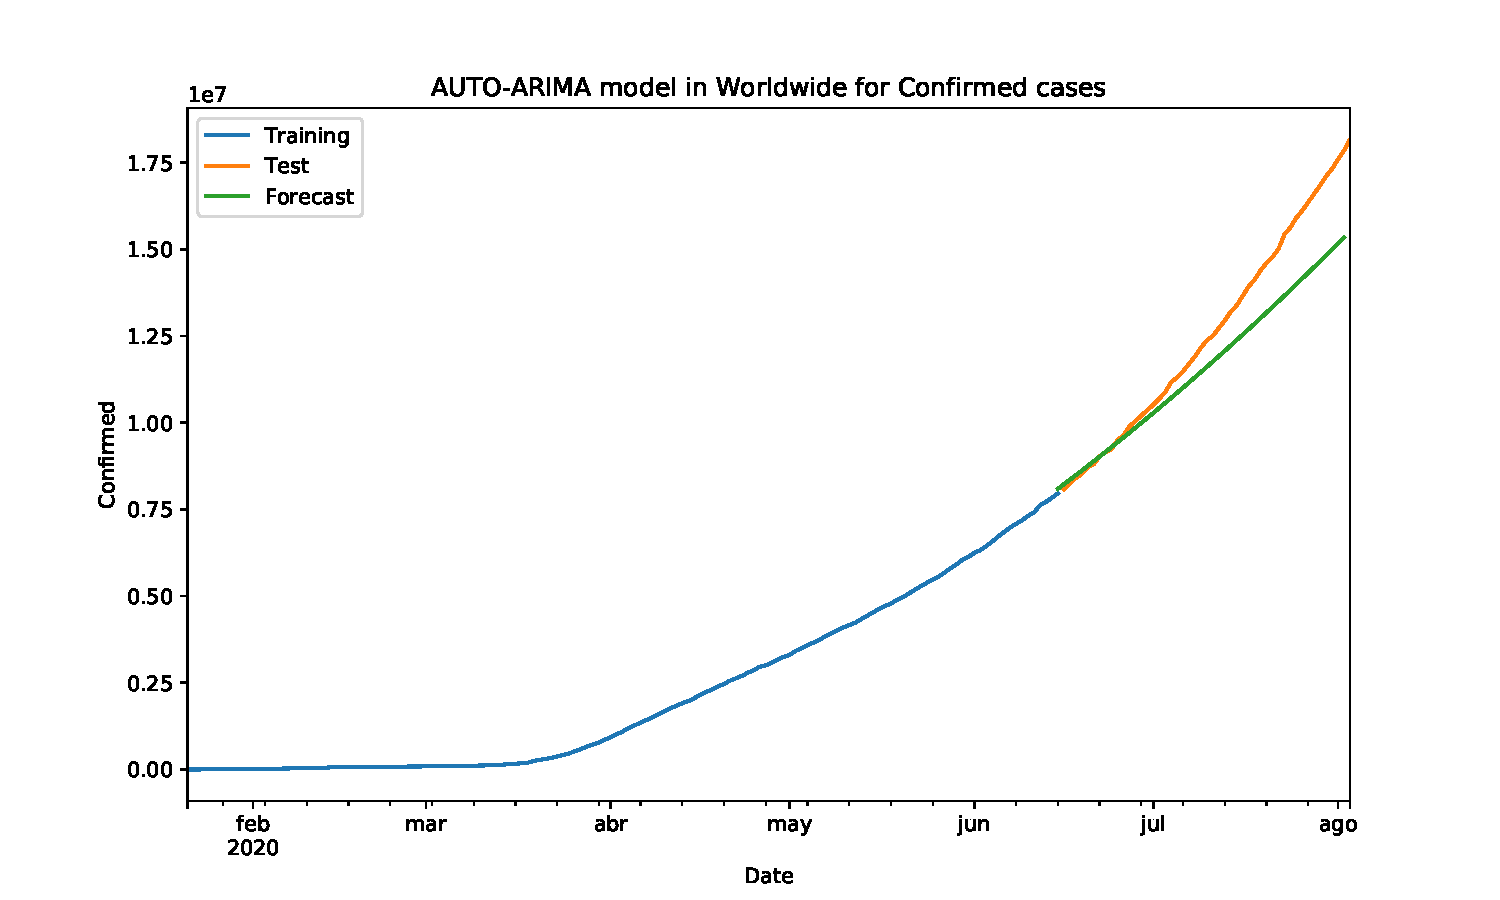
\includegraphics[scale=0.4]{plots/Worldwide_Confirmed_prediction.pdf}
        \caption{Prediction of confirmed cases in the world}
    \end{figure}
    
\end{itemize}

% Compare with other published works and detail any shortcomings of your work!
\section{Conclusion}
The model developed allowed us to get a quick intuition for any region in the world respect of the management of the crisis. The prediction shows us how the spreading will be progressed if any action would not be taken in order to deal with the spreading. Then we can compare the forecast values with the actual ones.

With this simple approach, it can be seen how well we faced the emergency. It reflects which regions have applied better measures and in which environments (number of cases respect population). Consequently, these results helps us to find better or more optimized ways to confront the new cases or being prepared for new waves in the future.

In addition to, we can see how the spreading of virus progress and the impact. Taking into account the confirmed cases, we are able to perform an analysis in how the virus evolve. Besides that, the number of deaths and recovered cases indicate us the rate of mortality and recuperation of COVID-19.

Future work could be develop more personalized models which fit better in each region, since it has been the main problem with our general approach. In spite of that, we have gotten good results in the test set for most of the regions.



\newpage
\bibliographystyle{unsrt}
\bibliography{references}

\end{document}
